% REMEMBER TO SET LANGUAGE!
\documentclass[a4paper,12pt,norsk]{article}
\usepackage[utf8]{inputenc}
% Standard stuff
\usepackage{amsmath,amsthm, amssymb,graphicx,varioref,verbatim,amsfonts,geometry,esint,url}
% colors in text
\usepackage[usenames,dvipsnames,svgnames,table]{xcolor}
% Hyper refs
\usepackage[colorlinks]{hyperref}
\usepackage{float}
\usepackage{wrapfig}
\usepackage{multicol}

\usepackage[export]{adjustbox}

\usepackage{subfig}

% Document formatting
\setlength{\parindent}{0mm}
\setlength{\parskip}{1.5mm}

%Color scheme for listings
\usepackage{textcomp}
\definecolor{listinggray}{gray}{0.9}
\definecolor{lbcolor}{rgb}{0.9,0.9,0.9}

\usepackage{listings}
\lstset{
	backgroundcolor=\color{lbcolor},
	tabsize=4,
	rulecolor=,
	language=python,
        basicstyle=\scriptsize,
        upquote=true,
        aboveskip={1.5\baselineskip},
        columns=fixed,
	numbers=left,
        showstringspaces=false,
        extendedchars=true,
        breaklines=true,
        prebreak = \raisebox{0ex}[0ex][0ex]{\ensuremath{\hookleftarrow}},
        frame=single,
        showtabs=false,
        showspaces=false,
        showstringspaces=false,
        identifierstyle=\ttfamily,
        keywordstyle=\color[rgb]{0,0,1},
        commentstyle=\color[rgb]{0.133,0.545,0.133},
        stringstyle=\color[rgb]{0.627,0.126,0.941}
        }
        
\DeclareMathOperator{\dist}{dist}
\newcommand{\distx}{\dist x}
        
\newcounter{subproject}
\renewcommand{\thesubproject}{\alph{subproject}}
\newenvironment{subproj}{
\begin{description}
\item[\refstepcounter{subproject}(\thesubproject)]
}{\end{description}}

%Lettering instead of numbering in different layers
%\renewcommand{\labelenumi}{\alph{enumi}}
%\renewcommand{\thesubsection}{\alph{subsection}}

%opening

\title{Fys4150 Project 1}
\author{Aksel Graneng}

\begin{document}
\maketitle

\abstract{enter abstract here}

\section{Introduction}

\section{Theory}

\subsection{Vectorized second derivative}

	If we have a 1d data-set on the form:
	$$\vec{V(x)} = [v_0,\ v_1,\ \cdots,\ v_{n-1},\ v_{n},\ v_{n-1},\ \cdots] $$\\
	Then we can write the second derivative of the data-set as:
	$$f_n = -\frac{v_{n+1} + v_{n-1} - 2v_n}{\Delta x^2} $$\\
	Where $\Delta x$ is the change in variable we are derivating based on; usually time.\\
	\\
	Rather than calculating the second derivatives of this data-set individually, we can instead calculate them all at the same time using linear algebra.\\
	This can be done by finding a matrix $A$ such that
	$$A\vec{V} = \vec{f} $$\\
	Where:
	\begin{gather*}
	\vec{f} = \left[
	\begin{array}{c}
	2v_i - v_2\\
	-v_1 + 2v_2 - v_3\\
	\vdots\\
	-v_{n-1} + 2v_n -v_{n+1}\\
	-v_n + 2v_{n+1} - v_{n+2}\\
	\vdots
	\end{array}
	\right]
	\end{gather*}
	As multiplying $\vec{f}$ with $\frac{1}{\Delta x^2}$ would give us an array containing all the second derivatives. We can see that $\textbf{A}$ must be:
	\begin{gather*}
	\textbf{A} = \left[
	\begin{array}{ccccc}
	2 & -1 & 0 & 0 & \cdots\\
	-1 & 2 & -1 & 0 & \cdots\\
	0 & -1 & 2 & -1 & \cdots\\
	\vdots & 0 & -1 & 2 & -1
	\end{array}
	\right]
	\end{gather*}


	
\section{Method}
	\subsection{General linear equation solver}
	The first thing our program does is solve a set of general linear equations on the form $\textbf{A}\textbf{v} = \textbf{f}$. This is done by putting the matrix $\textbf{M}$ on row reduced echeleon form:
	\begin{gather*}
	\textbf{M} =  \left[
	\begin{array}{cccccc}
	b_1 & c_1 & 0 & 0 & \cdots f_1\\
	a_2 & b_2 & c_2 & 0 & \cdots f_2\\
	0 & a_3 & b_3 & b_3 & \cdots f_3\\
	\vdots & 0 & a_4 & b_4 & \cdots f_4
	\end{array}
	\right]
	\end{gather*}

	Where $\textbf{M}$ is a $n \times (n+1)$ matrix. This is generally quite simple to solve using forward and backward substitution, but when $n$ becomes very large (in my experience, larger than $10^5$) we get problems with memory as well as computation time, as the most simple row reduction algorithm has $2(n+1)n^2$ FLOPS.\\
	To avoid this problem, we use the fact that most of the elements in the matrix is zero. In fact, there are at most 4 elements in each row that isnt zero. By removing every element that is zero from the matrix (except one in for the first and last line), we get:

\begin{gather*}
	\textbf{M}^* = \left[
	\begin{array}{cccc}
	b_1 & c_1 & 0 & f_1\\
	a_2 & b_2 & c_2 & f_2\\
	\vdots & \vdots & \vdots & \vdots\\
	0 & a_n & b_n & f_n
	\end{array}
	\right]
	\end{gather*}

	So now we have a $n \times 4$ matrix which contains all the information we need.\\
	\\
	We now use forward substitution on $\textbf{M}^*$ just like we would on $\textbf{M}$, except this time we "roll" the next row every time we subtract, so that $b_i$ is subtracted from $a_{i+1}$ and $c_i$ is subtracted from $b_{i+1}$. At the same time, we are careful to subtract $f_i$ from $f_{i+1}$. This means that index notation must be used, rather than numpy.roll.\\
	This is done in a loop that has $n$ iterations. First it does 3 operations, one on each element in the row except for the first (which is zero), along with a division, to normalize it. Then it does 3 subtraction and multiplication operations on the next row.\\
	\\
	Next is backwards substitution. Again we use a loop with n iterations. Here we only do 2 subtractions and multiplications, on the last and second last element of each row.\\
	All in all, this sums up to 14 FLOPS.\\
	\\
	After it was done, the general linear equation solver was tested on:
	\begin{gather*}
		u''(x) = f(x)\\
		\\
		f(x) = 100e^{-10x}
	\end{gather*}
	Which has a closed-form solution:
	$$u(x) = 1 - (1 - e^{-10})x - e^{-10x} $$
	
\section{Results}
	\subsection{General linear equation solver}
	We tested the general linear equation solver for datapoints $n = 10,\ n= 100,\ n=1000$
	\begin{figure}[H]
		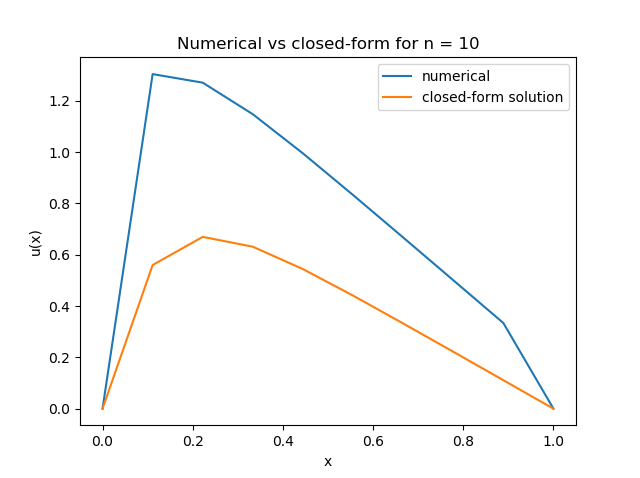
\includegraphics[scale = 0.7]{Figures/Figure_1.png}
		\centering
		\caption{The numerical solution vs the closed-form solution for 10 data-points. Here we can see that they deviate massively.}
	\end{figure}

	\begin{figure}[H]
		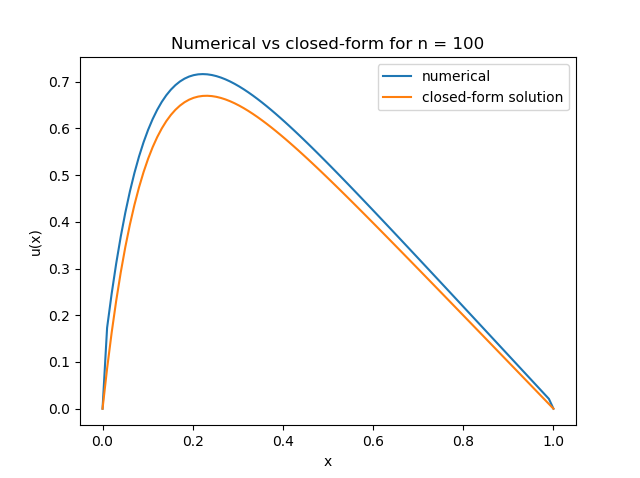
\includegraphics[scale = 0.7]{Figures/Figure_2.png}
		\centering
		\caption{The numerical solution vs the closed-form solution for 100 data-points. Here we can see that the difference is decreasing.}
	\end{figure}

	\begin{figure}[H]
		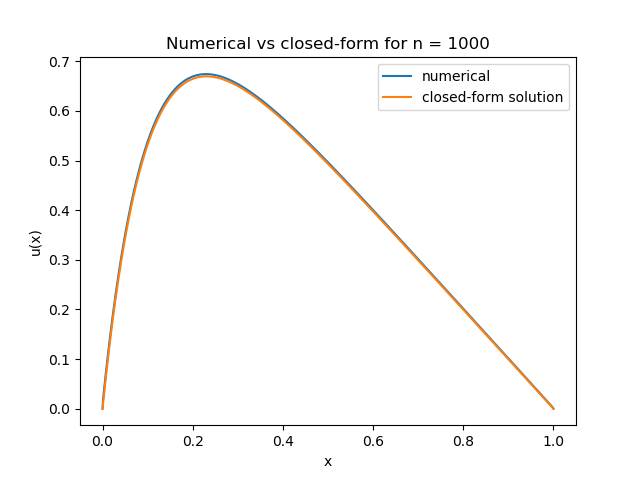
\includegraphics[scale = 0.7]{Figures/Figure_3.png}
		\centering
		\caption{The numerical solution vs the closed-form solution for 100 data-points. Here we can see that the difference has been even more decreased, and it is becoming hard to tell them apart.}
	\end{figure}
\section{Discussion}

\section{Conclusion}


\end{document}